\section{Results}

\begin{quote}
\textbf{Note on preliminary material.} The two studies below are \emph{preliminary} --- on a canonical
benchmark and an exploratory surface metric --- and fixed design choices carried into the rigorous
aerodynamic validation that follows. They are summarised compactly here; how each would be put on a
rigorous footing is set out in Section~\ref{sec:toward-rigour}.
\end{quote}

\subsection{Preliminary: representation and connectivity}

A canonical circle-series study fixed two design choices reused unchanged downstream: a single-scalar
radial node feature $[r]$ (rather than coupled Cartesian channels), and the ring-graph connectivity.
The connectivity was settled by an ablation sweeping the neighbours-per-side $k \in \{1, 2, 4, 6\}$ with
everything else fixed (4-layer GN, $T = 200$, 50 epochs), graded by the Kolmogorov--Smirnov (KS)
distance between the generated and reference radius distributions (lower is better).

% source: k-neighbour ablation, EXP-002, outputs/EXP-002{a,b,c,d}/evaluation_report.json
\begin{table}[t]
  \centering
  \begin{tabular}{lcc}
    \toprule
    Ring connectivity $k$ & KS statistic ($\downarrow$) & val loss \\
    \midrule
    1 (nearest-neighbour only) & 0.215          & 0.0642          \\
    2                          & 0.193          & 0.0403          \\
    4                          & 0.160          & 0.0414          \\
    6                          & \textbf{0.094} & \textbf{0.0378} \\
    \bottomrule
  \end{tabular}
  \caption{Ring-connectivity ablation on the circle benchmark (EXP-002): KS distance to the reference
  radius distribution and validation loss against neighbours per side $k$.}
  \label{tab:connectivity}
\end{table}

The KS distance falls monotonically with connectivity --- a 56\% reduction from $k = 1$ to $k = 6$,
corroborated by the validation loss --- so $k = 6$ was adopted for all downstream work. This is a
single-seed study on the circle benchmark, not an aerodynamic-domain result
(Section~\ref{sec:toward-rigour}).

\subsection{Preliminary: surface quality}
\label{sec:surface-quality}

Generated boundaries carry a small high-frequency wobble. An exploratory study swept six
training/sampling configurations against a mean second-difference roughness of $r(\theta)$ (lower is
smoother) on four fixed targets, to locate where surface quality is controlled.

% provisional
\begin{table}[t]
  \centering
  \begin{tabular}{lcccc}
    \toprule
    Configuration & Diffusion steps $T$ & Overall roughness & $\Delta$ vs baseline & Best val loss \\
    \midrule
    baseline                                        & 200  & 0.03379            & ---       & 0.00306   \\
    longer training                                 & 200  & 0.02125            & $-$37\%   & 0.000104  \\
    longer training $+$ $T=1000$ steps              & 1000 & \textbf{0.01523}   & $-$55\%   & 0.000090  \\
    $+$ Min-SNR-$\gamma$ loss \cite{hang2023minsnr} & 200  & 0.02700            & $-$20\%   & \textbf{0.000028} \\
    $+$ EMA \cite{song2020improved}                 & 200  & 0.03747            & $+$11\%   & 0.000124  \\
    $+$ EMA $+$ v-prediction \cite{salimans2022progressive} & 200 & 0.02451     & $-$27\%   & 0.000189  \\
    \bottomrule
  \end{tabular}
  \caption{Surface-quality sweep: roughness and validation loss for six training/sampling
  configurations. Lower roughness is smoother; bold marks the winner in each column.}
  \label{tab:surface-quality}
\end{table}

The single takeaway is that boundary smoothness is a \emph{sampling-time} property: the $T = 1000$
configuration roughly halves roughness ($-55\%$) while its validation loss is essentially unchanged from
longer-training-alone, and the lowest-loss configuration (Min-SNR-$\gamma$) is \emph{not} the smoothest.
Minimising the training MSE harder does not smooth boundaries --- more reverse-diffusion steps do. This
used a non-standard roughness proxy on four targets and is treated as exploratory; a rigorous
surface-quality protocol is outlined in Section~\ref{sec:toward-rigour}. Critically, the downstream
validation shows this wobble is cosmetic: it does not corrupt the measured physics
(Section~\ref{sec:in-dist}).

\subsection{CFD solver validation gate}
\label{sec:solver-gate}

Before trusting the loop on generated shapes, we gate it on \emph{known} dataset ellipses run with the
corrected domain --- the channel height $H$ taken from the dataset (5--6) with the body centred at the
half-height $H/2$, rather than the earlier free-chosen height.\footnote{An earlier preliminary gate
used a free-chosen channel height that did not match the dataset's domain; those runs are superseded by
the corrected-domain validation reported here.} The independent solver reproduces the
dataset's own $C_p$ at correlation up to $\approx 1.0$, establishing that the grading physics is sound
before any generated geometry is judged by it. The validation calculation interpolates the (monotonic)
dataset reference $C_p$ onto the solver's surface nodes --- the solver $C_p$ traces the full closed
boundary and is non-monotonic in $x/c$ --- and reports the Pearson correlation and the affine fit
$\mathrm{measured} \approx a\cdot\mathrm{ref} + b$.

\begin{table}[t]
  \centering
  \begin{tabular}{lcccccc}
    \toprule
    Sim & Re & $H$ & $C_p$ correlation & affine slope $a$ & offset $b$ \\
    \midrule
    sim\_59   & 503 & 5.5 & 0.971          & 1.76 & 0.06 \\
    sim\_2824 & 750 & 5.5 & 0.944          & 1.73 & 0.07 \\
    sim\_5645 & 998 & 5.5 & \textbf{0.999} & 1.87 & 0.02 \\
    \bottomrule
  \end{tabular}
  \caption{CFD solver validation gate on three known dataset ellipses spanning the Reynolds-number
  range at $H = 5.5$, with the corrected channel height: $C_p$ correlation, affine slope, and offset.}
  \label{tab:solver-gate}
\end{table}

The solver reproduces the dataset curve up to a single multiplicative normalisation $a \approx 1.7$--1.9,
strikingly close to the dataset's documented ``u / 1.8'' velocity scaling --- a credible analytic
explanation rather than a solver artefact --- with a near-zero offset $b$. Correlation dips slightly at
the mid-Reynolds case through genuine under-resolution of the stronger vortex shedding, not a
correctness failure.

\begin{figure}[t]
  \centering
  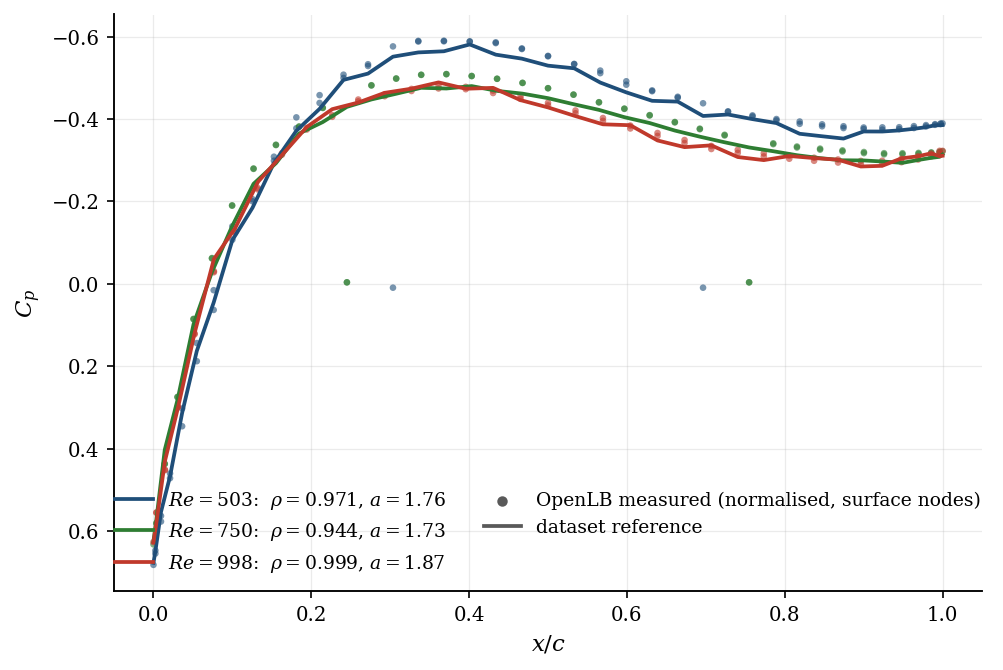
\includegraphics[width=0.8\linewidth]{EXP-043_cp_validation.png}
  \caption{Solver-measured surface pressure $C_p(x/c)$ (points, one per boundary node) against the
  dataset's own $C_p$ (solid lines) for three known ellipses spanning the Reynolds-number range at
  $H = 5.5$, with the corrected channel height. The measured nodes are mapped back into reference units
  by the per-case affine fit ($(\mathrm{measured} - b)/a$) so the shape agreement is shown directly; the
  amplitude $a \approx 1.7$--1.9 that is divided out --- the dataset's velocity normalisation --- is
  reported per curve in the legend.}
  \label{fig:cp-comparison}
\end{figure}

The measured $C_p$ is a time-average over a window spanning many shedding periods, and it is
well-converged: the per-node temporal RMS stays small ($\leq 0.12$) and the integrated drag is steady
($C_d = 0.86 \pm 0.06$), so the surface pressure the loop grades is a stable quantity rather than an
instantaneous snapshot.

\begin{figure}[t]
  \centering
  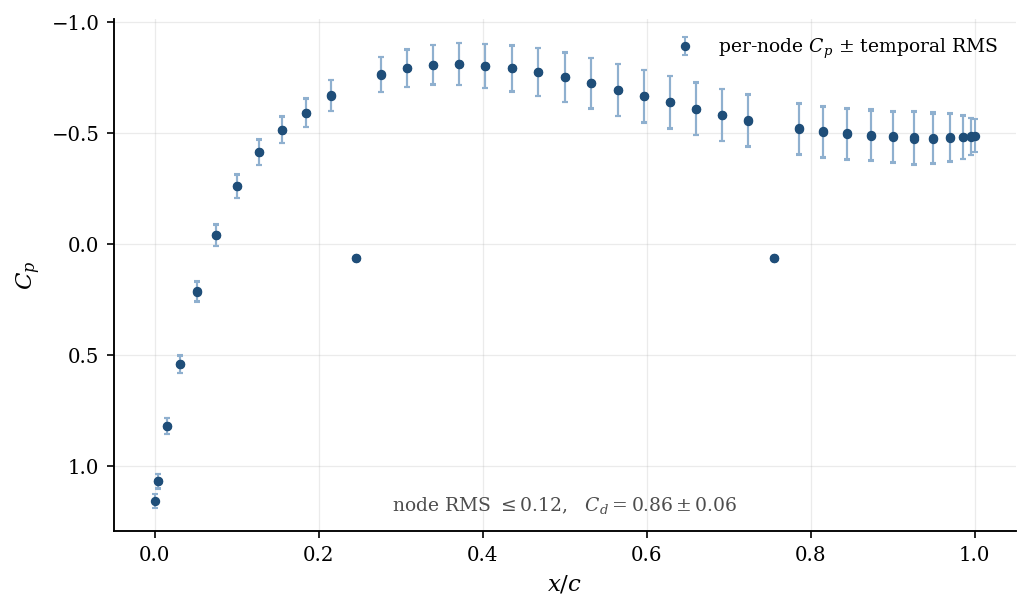
\includegraphics[width=0.8\linewidth]{EXP-043_cp_stability.png}
  \caption{Stabilisation of the surface $C_p$ for the mid-Reynolds case (Re = 750, $H = 5.5$): each
  marker is one boundary node's time-averaged $C_p$, with error bars showing the temporal RMS
  fluctuation over the averaging window. The small bands (node RMS $\leq 0.12$) and steady drag
  ($C_d = 0.86 \pm 0.06$) confirm the measured pressure is well-converged.}
  \label{fig:cp-stability}
\end{figure}

The three-ellipse spot-check is corroborated by a systematic gate over the whole design space. We
laid a 15-case grid across the dataset's $(Re, H)$ plane, snapping each grid node to its nearest real
simulation, and ran every case through the solver with per-case Reynolds-scaled resolution
($\mathrm{RES} \approx 0.2\,Re$); all 15 runs were numerically stable (no NaN, $\mathrm{avgRho}
\approx 1.0$, max CFL $\approx 0.1$).

\begin{table}[t]
  \centering
  \begin{tabular}{lcc}
    \toprule
    Quantity & Range across the 15-case grid & Mean \\
    \midrule
    $C_p$ correlation $\rho$ & 0.89 -- 1.00 & \textbf{0.96} \\
    affine slope $a$         & 1.51 -- 1.87 & \textbf{1.74} \\
    \bottomrule
  \end{tabular}
  \caption{Systematic 15-case solver-validation grid over the $(Re, H)$ design space: $C_p$
  correlation and affine slope range and mean.}
  \label{tab:eval-grid}
\end{table}

The mean slope $a \approx 1.74$ reproduces the three-ellipse normalisation ($a \approx 1.7$--1.9)
across the full $(Re, H)$ grid, confirming the single multiplicative factor is a stable property of the
solver --- the dataset's velocity normalisation --- and not an artefact of the three hand-picked cases.
With the gate holding at $\rho \approx 0.96$ everywhere in-distribution, \textbf{the solver is trusted
as physical ground truth for grading generated shapes.}

\begin{figure}[t]
  \centering
  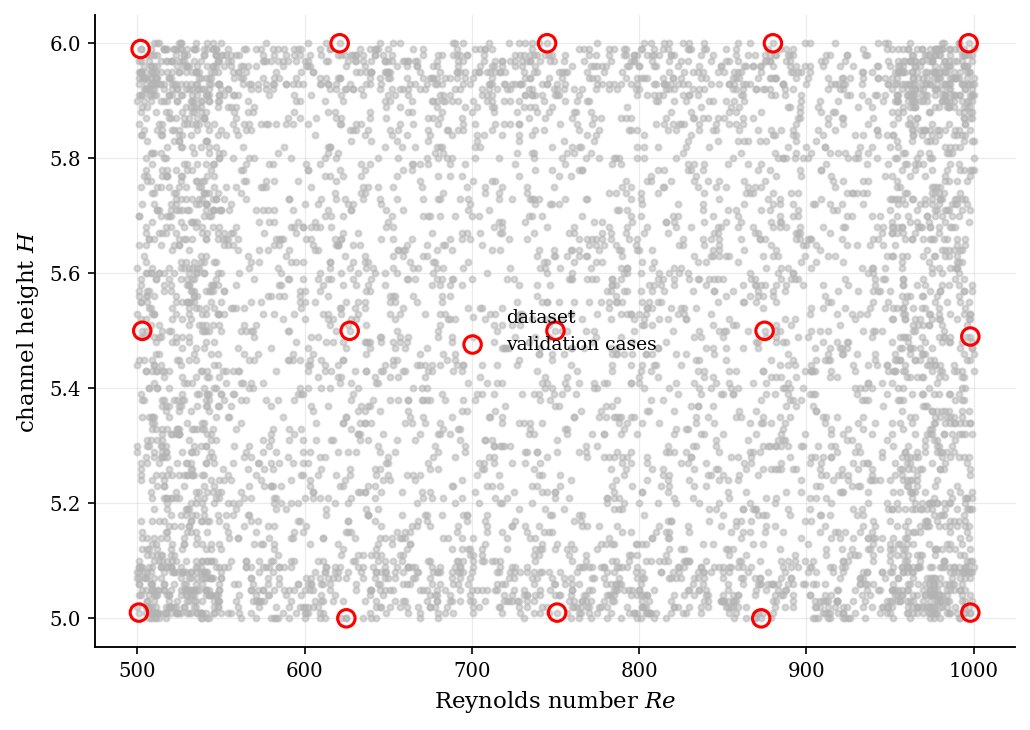
\includegraphics[width=0.8\linewidth]{EXP-043_eval_grid_coverage.png}
  \caption{The 15-case solver-validation grid laid over the training design space: each gate case
  (markers) is snapped to its nearest real simulation within the dataset $(Re, H)$ cloud, so the gate
  samples the whole regime rather than a few hand-picked points.}
  \label{fig:eval-grid-coverage}
\end{figure}

\subsection{In-distribution inverse design}
\label{sec:in-dist}

Generated shapes hit their target $C_p$ at correlation $\approx 0.95$ in-distribution, verified by
the independent solver rather than the model's own pressure head --- the first independent
confirmation of the inverse-design claim. Each shape is sampled for a dataset-drawn target $C_p$, run
through the validated loop, and its measured $C_p$ correlated against that target.

\begin{table}[t]
  \centering
  \begin{tabular}{lccc}
    \toprule
    Target & Re & $C_p$ corr (raw) & $C_p$ corr (smoothed) \\
    \midrule
    \#4849 & 960 & \textbf{0.964} & 0.952 \\
    \#4066 & 884 & \textbf{0.966} & 0.963 \\
    \bottomrule
  \end{tabular}
  \caption{In-distribution inverse-design validation: solver-measured $C_p$ correlation against the
  conditioning target for two generated shapes.}
  \label{tab:inverse-design}
\end{table}

Morphology is reproduced closely ($\rho \approx 0.95$--0.97), and the surface wobble of
Section~\ref{sec:surface-quality} proves cosmetic: raw versus Fourier-smoothed shapes differ by only
$\Delta\rho \sim 0.01$ in $C_p$ and $\sim 5\%$ in $C_d$, so it does not corrupt the measured physics.
Correlation --- not absolute amplitude --- is the verdict here: the model captures $C_p$ \emph{shape},
while its amplitude calibration (the affine slope) is a known limitation quantified on a controlled axis
in Section~\ref{sec:ood}.

\begin{figure}[t]
  \centering
  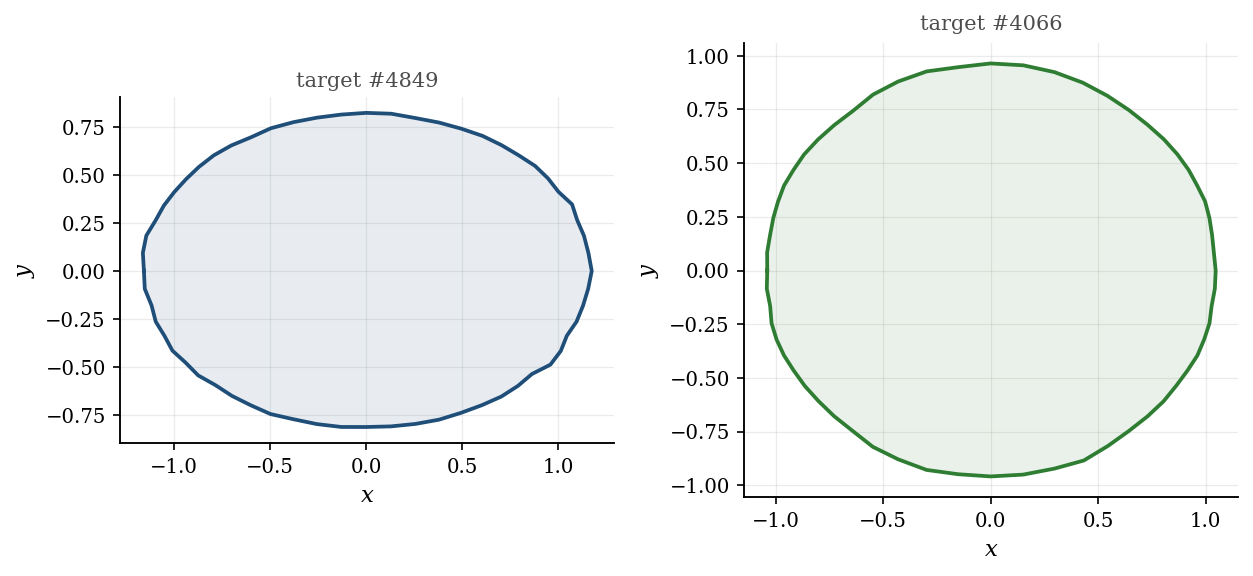
\includegraphics[width=0.8\linewidth]{report_generated_shapes.png}
  \caption{Boundaries generated by the conditional model for the in-distribution validation targets,
  before CFD grading.}
  \label{fig:generated-shapes}
\end{figure}

\begin{figure}[t]
  \centering
  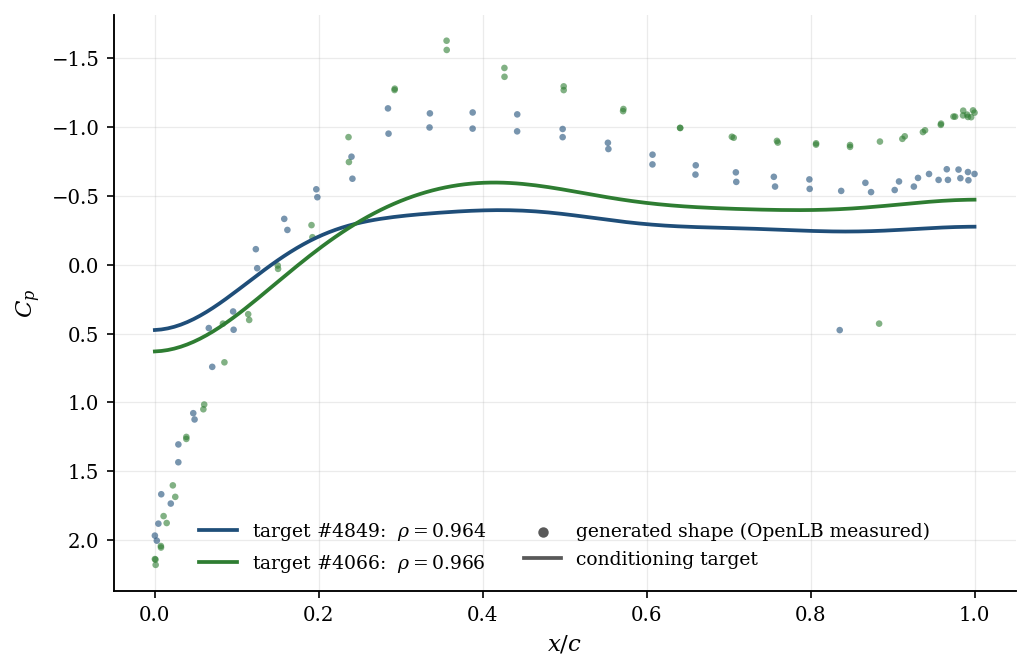
\includegraphics[width=0.8\linewidth]{EXP-041_cp_inverse_design.png}
  \caption{Solver-measured $C_p(x/c)$ of each generated in-distribution shape overlaid on its
  conditioning target: the morphology tracks closely.}
  \label{fig:cp-inverse-design}
\end{figure}

\subsection{Out-of-distribution behaviour and magnitude creep}
\label{sec:ood}

Out of distribution, inverse-design fidelity degrades --- the failure mode the independent loop was
built to surface. An initial five-target ad-hoc probe first exposed this; we report the
\textbf{controlled successor} that supersedes it. The OOD axis is made principled by perturbing the
dataset-mean $C_p$ along the dataset's own principal pressure modes,
\[
  C_p^{\mathrm{target}}(x) = \overline{C_p}(x) + s \cdot \alpha \cdot \sigma_m \cdot \mathrm{PC}_m(x),
\]
for modes $m \in \{\mathrm{PC1}, \mathrm{PC2}\}$, amplitudes $\alpha \in \{1, 2, 3, 4\}$ $\sigma$-units,
and both signs $s$ (16 targets). Each is generated with plain classifier-free guidance at fixed
$Re/H = 754/5.5$ --- so target morphology is the only variable --- and graded through the validated
solver (all 16 runs stable).

\begin{table}[t]
  \centering
  \begin{tabular}{cccc}
    \toprule
    amplitude $\alpha$ ($\sigma$) & OOD distance & $C_p$ corr $\rho$ & affine slope $a$ \\
    \midrule
    1 & 1.80 & 0.901          & 2.08 \\
    2 & 2.02 & 0.922          & 2.06 \\
    3 & 2.33 & 0.858          & 1.79 \\
    4 & 2.74 & \textbf{0.857} & 1.76 \\
    \bottomrule
  \end{tabular}
  \caption{The genuinely-OOD $+\mathrm{PC1}$ ladder: $C_p$ correlation and affine slope against
  out-of-distribution distance as the target amplitude is pushed from 1 to 4$\sigma$.}
  \label{tab:ood-ladder}
\end{table}

Along the genuinely-OOD $+\mathrm{PC1}$ direction, correlation falls monotonically from $\sim 0.92$ to
$\sim 0.86$ as the target moves out. One parameterisation caveat --- itself a finding --- is that
\textbf{only $+\mathrm{PC1}$ is genuinely reachable as OOD}: the other principal directions stay near
the training manifold (OOD distance $\approx 1.0$--1.6) regardless of amplitude, because the raw-curve
PCA $\sigma$-units are not isometric to the DCT-conditioning space the model sees. A future ladder
should sweep amplitude in conditioning space directly (Section~\ref{sec:toward-rigour}).

\begin{figure}[t]
  \centering
  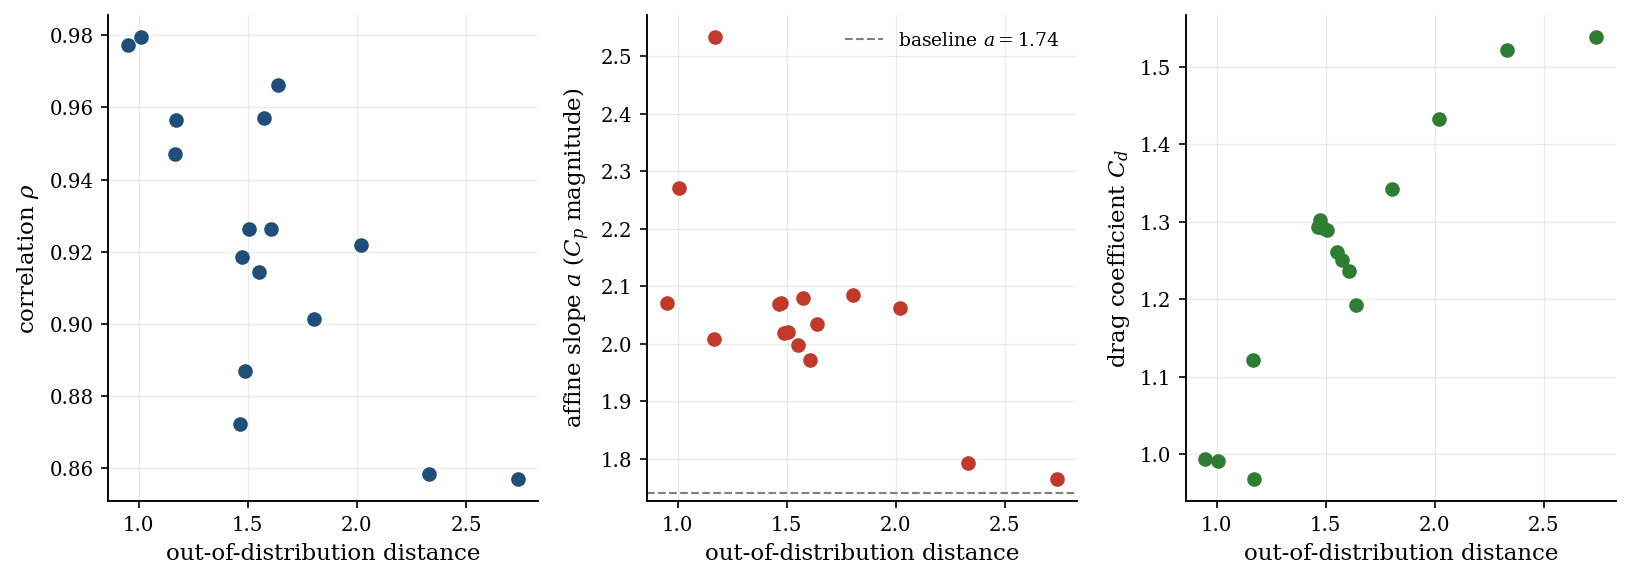
\includegraphics[width=0.95\linewidth]{EXP-043_ood_results_summary.png}
  \caption{Inverse-design fidelity against out-of-distribution distance across the 16-target ladder:
  correlation $\rho$ (left) softens, the affine slope $a$ (centre) sits above the validated 1.74
  baseline, and drag $C_d$ (right) rises with OOD distance.}
  \label{fig:ood-results-summary}
\end{figure}

\begin{figure}[t]
  \centering
  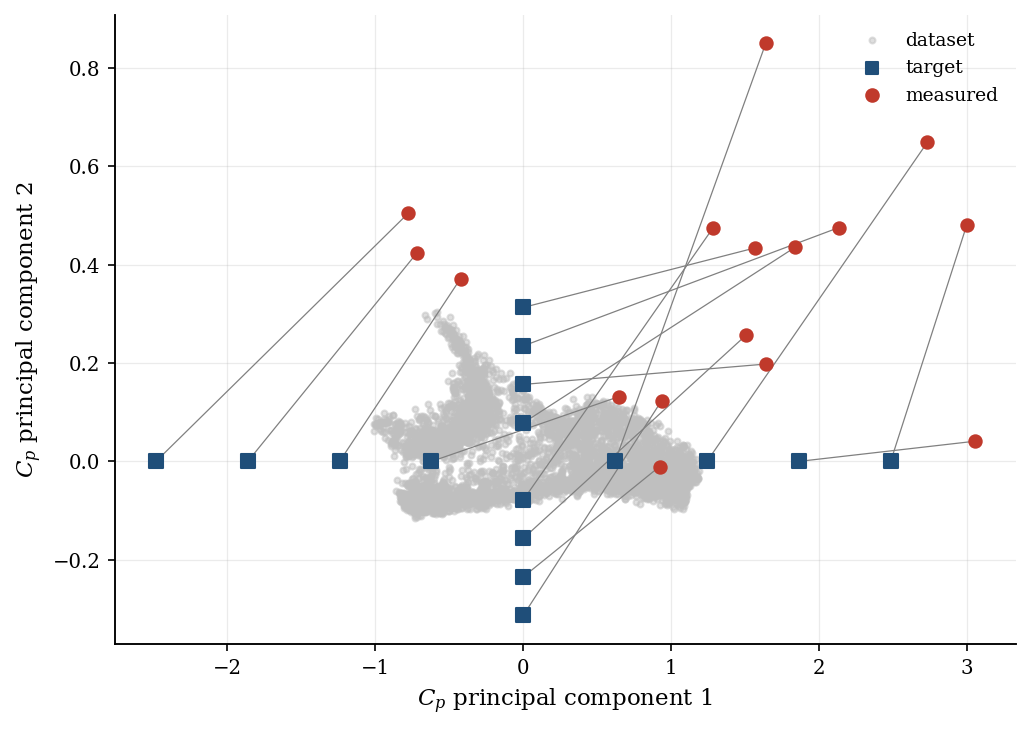
\includegraphics[width=0.8\linewidth]{EXP-043_ood_cp_manifold.png}
  \caption{The OOD ladder in the dataset's principal-component $C_p$ plane: training curves form the
  backdrop cloud; the $+\mathrm{PC1}$ targets march progressively outside it (making
  ``out-of-distribution'' concrete), while the other directions stay near the training manifold.}
  \label{fig:ood-cp-manifold}
\end{figure}

\paragraph{The amplitude bias is model-side.} Across all 16 OOD targets the affine slope spans
$a \approx 1.8$--2.5, above the solver's validated in-distribution baseline of 1.74
(Section~\ref{sec:solver-gate}). The point is sharpest when real dataset shapes and generated shapes are
graded by the \emph{same} solver: dataset ellipses sit at the validated baseline ($a \approx 1.6$--1.8),
while generated shapes --- in-distribution and out-of-distribution alike --- sit well above it
($a \approx 2.5$--3.5). A separate resolution- and node-density-controlled study further confirms $a$ is
unmoved by any CFD or discretisation lever. The creep is therefore a generative amplitude bias
(pressure-head calibration), to be closed model-side with the solver trusted as ground truth, not a
discretisation artefact.

\begin{figure}[t]
  \centering
  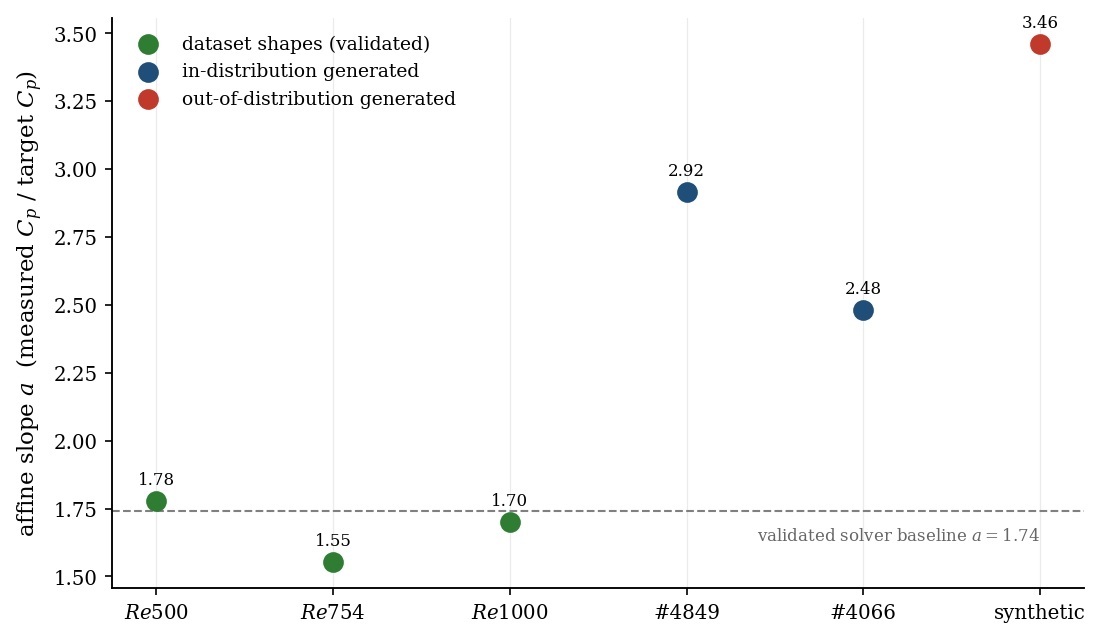
\includegraphics[width=0.8\linewidth]{EXP-042_creep_ladder.png}
  \caption{Affine slope $a$, graded by the same solver, from validated dataset shapes to generated
  shapes: real dataset ellipses sit at the validated baseline ($a \approx 1.6$--1.8, dashed), while
  generated shapes --- in-distribution (\#4849, \#4066) and out-of-distribution (synthetic) --- sit well
  above it ($a \approx 2.5$--3.5), isolating the magnitude creep to the generator.}
  \label{fig:creep-ladder}
\end{figure}

\paragraph{Posterior guidance is the wrong knob out of distribution.} The intuitive fix --- Diffusion
Posterior Sampling \cite{chung2023dps}, adding a likelihood gradient from the model's own pressure head
--- makes every metric worse, swept on a fixed OOD target at constant seed so the shapes differ only by
the guidance:

\begin{table}[t]
  \centering
  \begin{tabular}{lccc}
    \toprule
    DPS weight & $C_p$ corr & affine slope $a$ & $C_d$ \\
    \midrule
    0.0 (plain CFG) & \textbf{0.860} & 3.46 & 1.59 \\
    0.3             & 0.818          & 5.22 & 2.46 \\
    0.5             & 0.807          & 5.32 & 2.33 \\
    1.0             & 0.762          & 6.48 & 3.10 \\
    \bottomrule
  \end{tabular}
  \caption{DPS guidance sweep on a fixed out-of-distribution target: $C_p$ correlation, affine slope,
  and drag coefficient all degrade monotonically with guidance weight.}
  \label{tab:dps-sweep}
\end{table}

Correlation falls while the amplitude slope and drag rise monotonically: DPS steers toward the
self-trained pressure head, which is exactly the unreliable component out of distribution, so stronger
guidance optimises the surrogate's own error. Plain classifier-free guidance is the correct OOD
configuration; the gap is not closable by a self-graded posterior.

\begin{figure}[t]
  \centering
  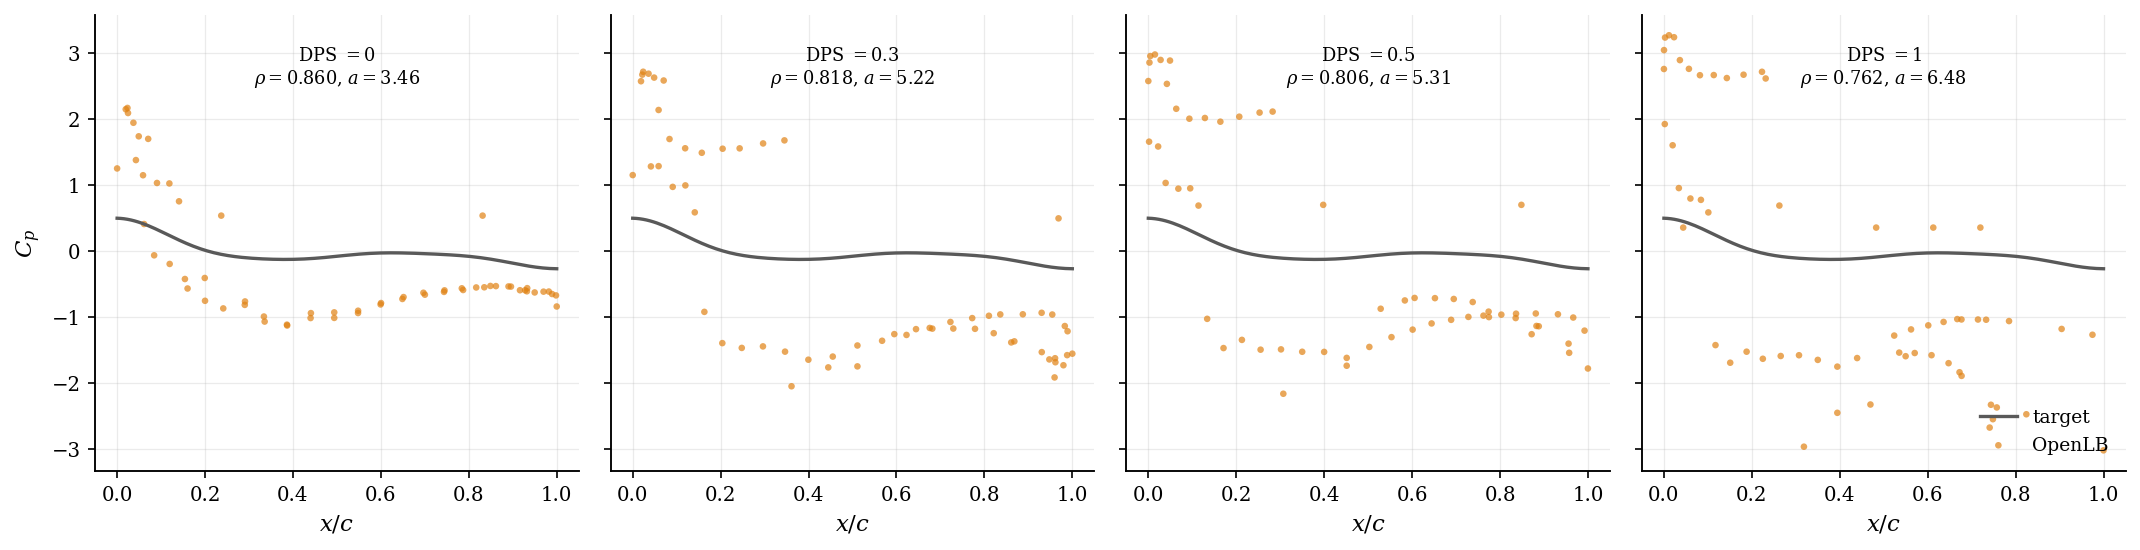
\includegraphics[width=0.8\linewidth]{EXP-041_dps_sweep.png}
  \caption{Inverse-design fidelity against DPS guidance weight: correlation falls while the amplitude
  slope and drag rise monotonically, so posterior guidance degrades true out-of-distribution fidelity.}
  \label{fig:dps-sweep}
\end{figure}

\subsection{Qualitative flow fields}

Instantaneous OpenLB fields around a generated in-distribution shape, rendered in ParaView, give
the qualitative picture behind the validation numbers. In the velocity-magnitude field the laminar
boundary layer separates off the body and rolls up into a regular von K\'{a}rm\'{a}n vortex street
--- the alternating wake that defines the Re 500--1000 shedding regime --- with accelerated flow
over the shoulders and a low-momentum wake behind the body.

\begin{figure}[t]
  \centering
  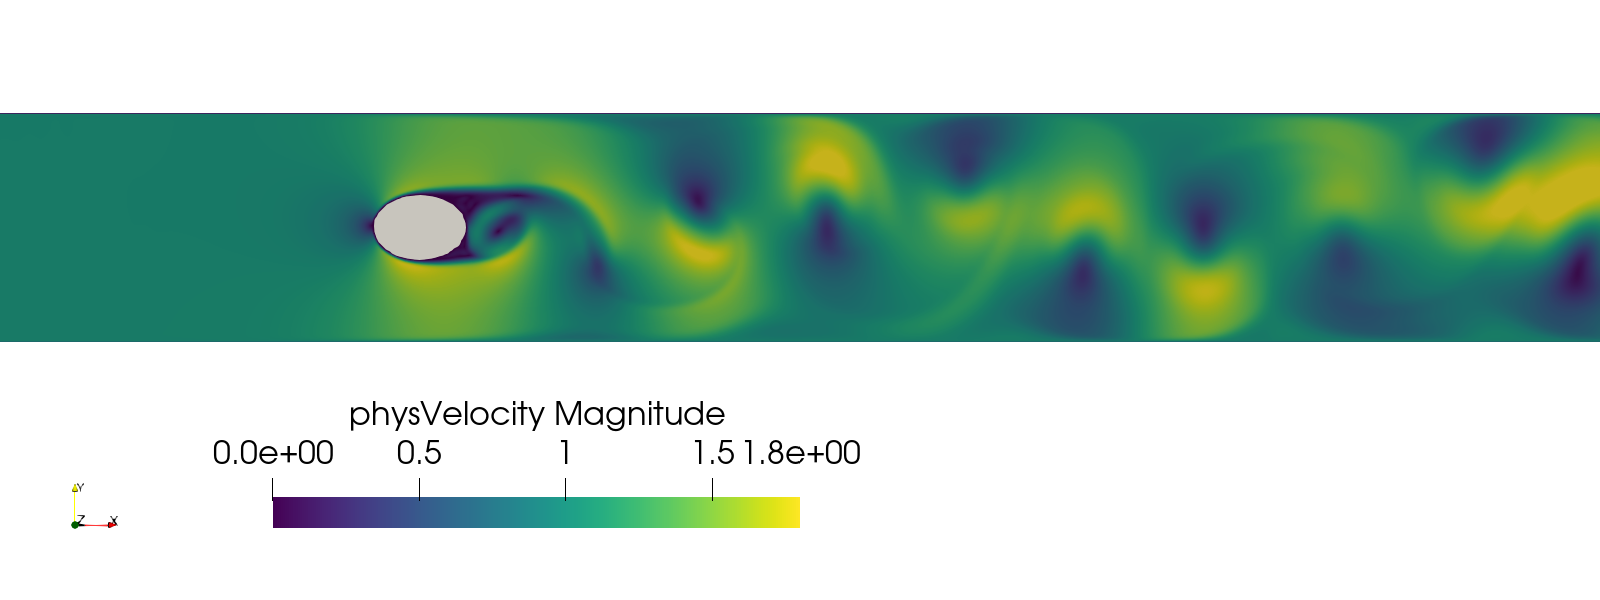
\includegraphics[width=0.8\linewidth]{report_paraview_velocity_wake.png}
  \caption{Velocity-magnitude field around a generated in-distribution shape: a laminar separation
  rolling up into a regular von K\'{a}rm\'{a}n vortex street, with accelerated shoulder flow and a
  low-momentum wake.}
  \label{fig:paraview-velocity}
\end{figure}

The pressure field at the same instant shows a high-pressure stagnation region on the upstream nose
and a train of discrete low-pressure vortex cores shed into the wake. The surface trace of exactly
this field \emph{is} the $C_p(x/c)$ curve that the inverse-design loop grades, making concrete what
the correlation numbers above are measuring.

\begin{figure}[t]
  \centering
  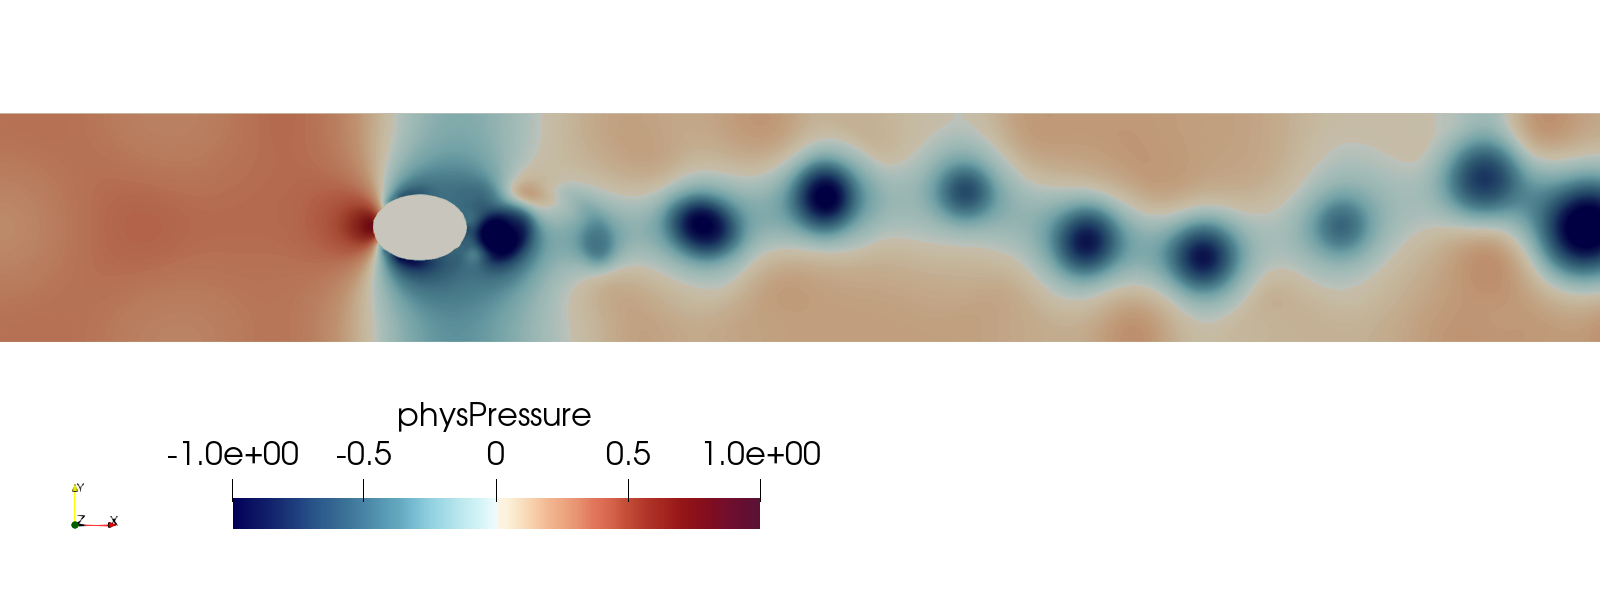
\includegraphics[width=0.8\linewidth]{report_paraview_pressure.png}
  \caption{Pressure field at the same instant: a high-pressure stagnation nose and a train of
  discrete low-pressure vortex cores in the wake, whose surface trace is the graded $C_p(x/c)$
  curve.}
  \label{fig:paraview-pressure}
\end{figure}
